\documentclass{article}
\usepackage[utf8]{inputenc}
\usepackage[letterpaper, margin=1in]{geometry}
\usepackage{pgfplots}

\title{Miniproyecto FADA - Universidad del Valle}
\date{}
\author{David Santiago Cortés, Alejandro Orozco, Brayan Rincones}

\begin{document}
	\maketitle

	\section{Soluciones Planteadas}
		\textbf{Idea General de la solución:}\\
		Almacenar los animales y sus grandezas en una estructura de datos tipo lista, arreglo o diccionario, 
		se ordena esta estructura de acuerdo a los valores de las grandezas y se guarda utiliza para armar las
		escenas de todas las partes del evento.\\	
		\subsection{$O(n^2)$}
			\textbf{Idea de la solución:} una vez que obtenemos el archivo lo descomponemos para obtener los valores de n, m, k, los animales participantes con sus grandezas, la apertura y las partes. Los animales participantes y grandeza se guardaron en un diccionario con los nombres de los animales como keys, las partes y la apertura como listas, y n,m, y k como enteros. Después se procedió de la siguiente forma:
			\begin{enumerate}
				\item Apertura: para ordenar la apertura primero ordenaremos las escenas de la apertura, la manera en la que se ordena consiste en dos bucles que van recorriendo la lista comparando, esta lista la guardamos en un lista auxiliar, en la lista ya arreglada usamos un bucle para recorrer las escenas y ordenarlas en términos de la grandeza de los animales.
				\item Partes: primero ordenaremos las partes por su grandeza total, después recorreremos la lista y ordenaremos cada parte internamente por la grandeza de la escena y por último se ordenan por la grandeza de los animales.
				\item Explicación para resolver las apariciones, la escena de más/menos grandeza y el promedio: ya que la apertura tiene $(m-1)*k$ escenas y las partes combinadas todas tienen $(m-1)*k$ escenas, como también está la condición de que todas las escenas de las partes están en la apertura y viceversa. con esta premisa procederemos a resolver las apariciones, la escena de más/menos grandeza y el promedio.
				\item Apariciones de animales: para saber qué animal apareció más/menos primero se "desencadenara" la lista de la apertura, para después encontrar que elemento se repite más/menos, sabiendo que elemento se repita más/menos usamos un bucle para contar cuantas veces aparece, y después con el número que obtenemos buscamos otros elementos que se repitan la misma cantidad de veces, por último eliminamos los elementos repetidos. El número de apariciones de un animal en el evento es de $2*apariciones$ en la apertura usando la premisa del punto 3.
				\item Escenas de mayor/menor grandeza: usando también la premisa del punto 3 sabemos que la escena de mayor/menor grandeza del evento será la misma que de la apertura, entonces cuando se organizó la apertura en 1, simplemente para el mayor valor se obtuvo el último valor de la lista y para el menor valor se obtuvo el primer valor de la lista.
				\item Promedio grandeza: al igual que 4 y 5 se usa la premisa 3. el  promedio de el evento es de 
				\begin{equation}
					p=\frac{2*grandezaApertura}{2*(m-1)*k} \rightarrow p=\frac{grandezaApertura}{(m-1)*k}
				\end{equation}
				en otras palabras el promedio de la apertura. Para sacar el promedio se usó una variable la cual hace uso de un bucle para recorrer la apertura y sumar la grandeza de cada animal y al final se divide por $(m-1)*k$
			\end{enumerate}
			\textbf{Estructuras de datos utilizadas:} Listas, Diccionarios\\ 
			\textbf{Algoritmo de ordenamiento:} Bucles\\
			\textbf{Lenguaje en el que se implementó:} Python
		
		\subsection{$O(n*\log(n))$}
			\textbf{Idea de la solución:}
			En la descripción del problema tenemos una serie de elementos que, de alguna manera, hay que ordenarlos para dar con el espectáculo 
			final. Al tener que organizar ascendentemente los escenarios de acuerdo a las grandezas de cada animal, además de organizar las partes
			acorde a las grandezas de las escenas que conlleva, se considera que este problema se puede llevar a cabo mediante el ordenamiento de Merge Sort,
			cuando ya tengamos definido las características de los animales, estos serán almacenados en arreglos, tanto nombres en un arreglo, 
			como grandezas respectivas en otro arreglo, los cuales serán los datos de entrada.\\
			Ya organizados los animales en un escenario por una función auxiliar, esta misma es llamada dentro del Merge Sort,
			con esto estamos organizando las partes finales acorde a operaciones como tamaños de medias de grandezas de los escenarios. 
			Extrayendo los datos, podemos obtener la media total de grandeza, el animal que mas participo, escena de mayor grandeza, 
			menor grandeza así como el que menos lo hizo mediante contadores, abstracción y almacenamiento en nuevos arreglos de 
			los resultados finales, cada operación con su respectiva función dentro del algoritmo.\\\\
			\textbf{Estructuras de datos utilizadas:} \\
			\textbf{Algoritmo de ordenamiento:}Merge Sort\\
			\textbf{Lenguaje en el que se implementó:} Python\\
		\subsection{$O(n)$}
			\textbf{Idea de la solución:} Después de recolectar los datos de entrada se construye un diccionario que mapea 
			animales a sus respectivas grandezas a partir de la lista de animales y grandezas que se pasaron como parametro de
			entrada. Este diccionario se usará más adelante para apoyar distintas operaciones.\\
			Para atacar el problema se utiliza una estrategia \textit{bottom-up} 
			\begin{enumerate}
				\item Ordenar las escenas localmente: para que todas las escenas del evento queden ordenadas localmente solo basta con ordenar
					las escenas de la apertura. El ordenamiento se hace con una implementación de Counting Sort que ordena una lista de 
					tuplas (animal,grandeza) en orden ascendente de acuerdo a las grandezas. 
				\item Ordenar las escenas de las demás partes (localmente): con el resultado del paso anterior se construye un diccionario/tabla hash
					que relaciona escenas desordenadas con escenas ordenadas, se usa un ciclo que itera sobre cada escena de las m-1
					partes y se reemplaza cada escena en cada parte haciendo la consulta en la tabla hash.
				\item Ordenar todas las escenas: teniendo todas las escenas ordenadas localmente en cada parte, lo que resta es ordenar las escenas
					dentro de sus partes de acuerdo a sus grandezas. El proceso se divide en dos, la primera parte
					se encarga de constuir un diccionario/tabla hash que relacione escenas con su grandeza, para ello se itera sobre 
					apertura y se calcula la grandeza de cada escena, con esta información ordenamos apertura utilizando Counting Sort.\\
					En la segunda parte se itera sobre las siguientes $m-1$ partes y sobre las $k$ escenas de tales partes, se consulta cada escena
					en el diccionario para hallar su grandeza y antes de cambiar a la siguiente parte, se ordenan las escenas de la parte actual
					con Counting Sort. Al finalizar el ciclo externo las escenas dentro de cada parte están ordenadas ascendentemente.

					\begin{enumerate}
						\item Empates: se buscan y se resuelven cada que se ordenan las escenas de una parte. Para detectarlos se usa una función
							que detecta duplicados en una lista utilizando la librería \texttt{collections}. Una vez se saben los indices de los 
							elementos repetidos, se utiliza la función \texttt{remove\_duplicates} que remueve los duplicados con un \texttt{while}
							que va "en reversa" empezando en $i=2$ hasta $0$, $i$ se usa para acceder una tabla hash que mapea animales a grandezas.

					\end{enumerate}
				\item Ordenar las partes: para ordenar las partes es necesario saber las grandezas de cada parte, lo cual se hace en el paso
					anterior cada que se va iterando sobre cada parte y se van almacenando los valores una en una lista. \texttt{sort\_parts}
					entonces fusiona las $m-1$ partes con sus grandezas, generando una lista de tuplas (parte, grandeza) que se le pasa
					como parametro a la función de ordenar.
				\item Estadísticas del evento: 
					\begin{enumerate}
						\item Animal más popular y menos popular: se utiliza una lista de todas
						las escenas que ocurren en el evento (con apertura y las demás partes) y la lista de animales del evento. Con ambas se construye
						una tabla hash que mapea animales a número de veces que aparecieron en escena, como candidato para animal más popular y menos popular
						se tiene obviamente al elemento máximo y mínimo de los valores de la tabla hash, para no dejar por fuera ningún otro animal
						se itera sobre la tabla hash buscando animales distintos al candidato y cuyas apariciones sean iguales a las del candidato. 
						\item Promedio de grandeza del evento: se itera sobre la lista de todas las escenas que tuvieron lugar, se suman sus grandezas
							y se divide entre el número de escenas que se mostraron. Lo mismo también puede lograrse con las partes y sus grandezas.

						\item Escenas de mayor y menor grandeza: se calcula el elemento más grande y más pequeño en la tabla hash que mapea escenas
							a sus grandezas.
					\end{enumerate}
			\end{enumerate}
			\textbf{Estructuras de datos utilizadas:} Listas, tablas hash, tuplas\\
			\textbf{Algoritmo de ordenamiento:} Counting Sort para listas de tuplas (animal, grandeza)\\
			\textbf{Lenguaje en el que se implementó:} Python
	\section{Análisis de Resultados}
		\subsection{$O(n^2)$}
            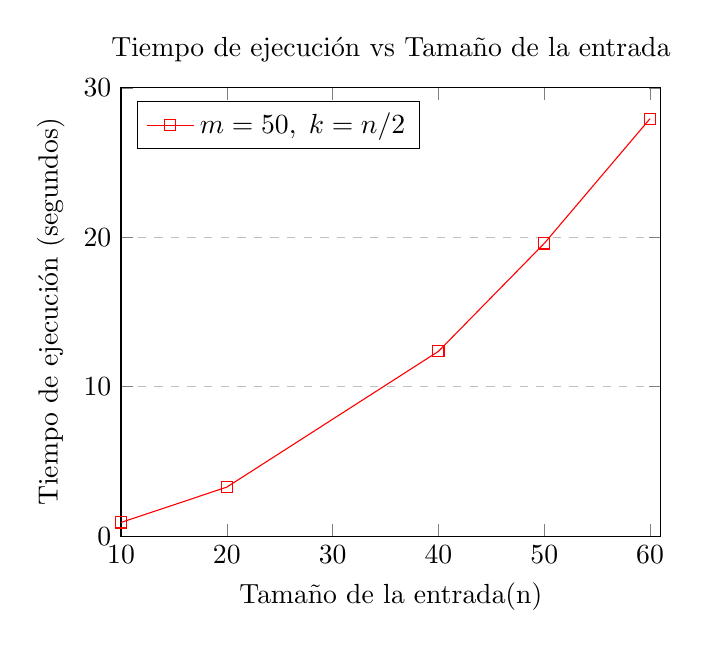
\begin{tikzpicture}
            \begin{axis}[
                title={Tiempo de ejecución vs Tamaño de la entrada},
                xlabel={Tamaño de la entrada(n)},
				ylabel={Tiempo de ejecución (segundos)},
                xmin=10, xmax=61,
				ymin=0, ymax=30,
                xtick={},
                ytick={},
                legend pos=north west,
                ymajorgrids=true,
                grid style=dashed,
            ]
            
            \addplot[
                color=red,
                mark=square,
                ]
                coordinates {
					(10,0.918)(20,3.284)(40,12.37)(50,19.591)(60,27.941) 
                };
				\addlegendentry{$m=50,\; k=n/2$}
            \end{axis}
            \end{tikzpicture}
		\subsection{$O(n*\log(n))$}
			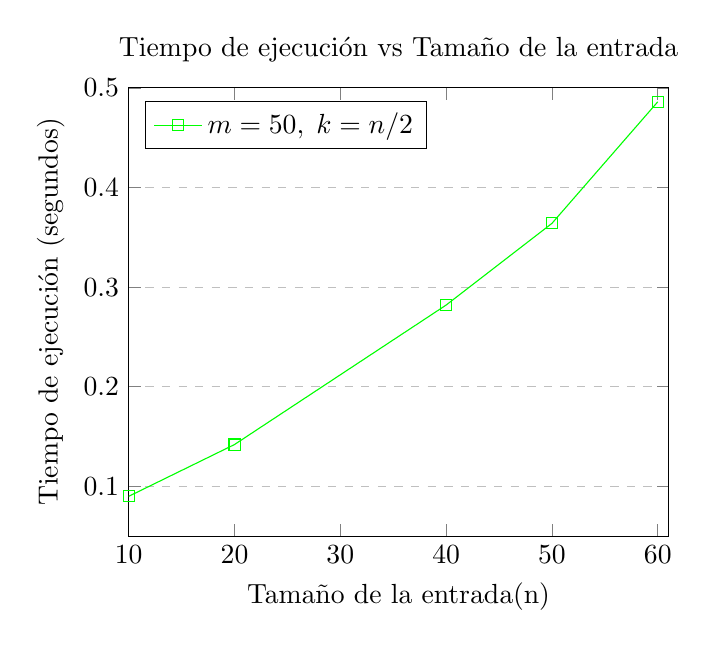
\begin{tikzpicture}
				\begin{axis}[
					title={Tiempo de ejecución vs Tamaño de la entrada},
					xlabel={Tamaño de la entrada(n)},
					ylabel={Tiempo de ejecución (segundos)},
					xmin=10, xmax=61,
					ymin=0.05, ymax=0.5,
					xtick={},
					ytick={},
					legend pos=north west,
					ymajorgrids=true,
					grid style=dashed,
					]
					\addplot[
					color=green,
					mark=square,
					]
					coordinates {
						(10,0.09)(20,0.142)(40,0.282)(50,0.364)(60,0.486)
					};
					\addlegendentry{$m=50,\; k=n/2$}
				\end{axis}
			\end{tikzpicture}
		\subsection{$O(n)$}
			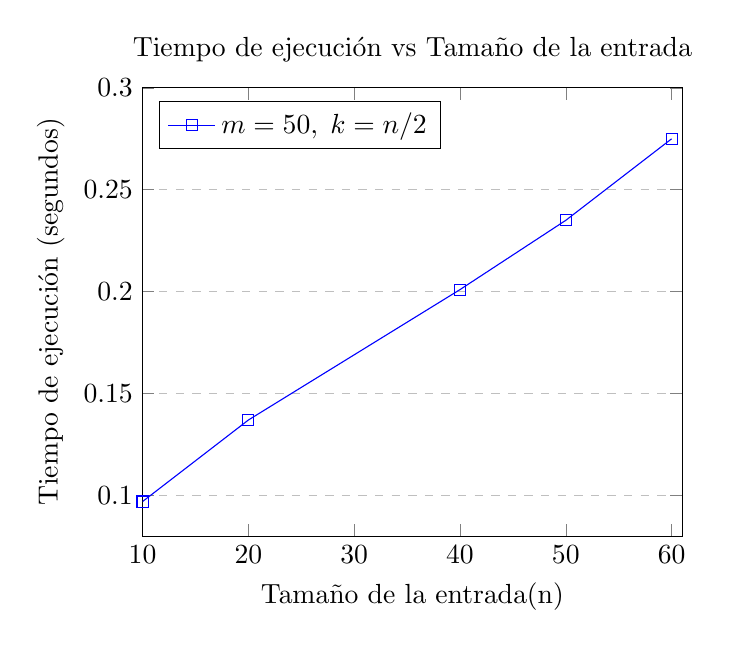
\begin{tikzpicture}
				\begin{axis}[
					title={Tiempo de ejecución vs Tamaño de la entrada},
					xlabel={Tamaño de la entrada(n)},
					ylabel={Tiempo de ejecución (segundos)},
					xmin=10, xmax=61,
					ymin=0.08, ymax=0.3,
					xtick={},
					ytick={},
					legend pos=north west,
					ymajorgrids=true,
					grid style=dashed,
					]
					\addplot[
					color=blue,
					mark=square,
					]
					coordinates {
						(10,0.097)(20,0.137)(40,0.201)(50,0.235)(60,0.275)
					};
					\addlegendentry{$m=50,\; k=n/2$}
				\end{axis}
			\end{tikzpicture}
		\section[title]{Instrucciones para la ejecución\footnote{Si se quiere utilizar una entrada propia, por favor revisar el formato de las entradas ya hechas.}}
		\subsection{$O(n^2)$}
		En la linea de comandos o al final del programa escribir zoo("nombre del archivo a ejectura")
		\subsection{$O(n*\log(n))$}		
		Ya por defecto existe una entrada en la carpeta de archivos, \texttt{entrada.txt}, con datos muy grandes para la prueba del programa solZoonlogn.py, puesto que no se notan cambios muy bruscos con respecto al tiempo de ejecución final al probar con datos de entrada pequeños. 
		Por ende, como ya hay un archivo de entrada, se procede a ejecutar el programa (run) \texttt{solZoonlogn.py} desde una ide de python3 o por medio de terminal pasandole como argumento el nombre y la ruta al archivo de entrada y este retorna los resultados por consola.\\\\
		Si desea cambiar y probar con otra entrada, el archivo \texttt{file.py} es un programa que modifica a entrada.txt, con los valores para n,m,k, animales y grandezas que usted elija, inclusive en este documento encontrará tests con los cuales hemos probado, con sus respectivas medidas de tiempo de ejecución. Si quiere modificar la entrada manualmente, aquí hay algunos ejemplos de pruebas realizadas con anterioridad, solo tiene que copiar alguno de estos ejemplos en el archivo de entrada.txt y así reemplazar el contenido que esté ya tenía.
		\subsection{$O(n)$}
			\texttt{./run.py <nombre-archivo-entrada>}
	\section{Sets de prueba}
		Se encuentran dentro de la carpeta \texttt{/entradas}
	\section{Conclusiones del proyecto}
	\begin{enumerate}
		\item Al comparar los resultados obtenidos usando los diferentes algoritmos para ordenar se encuentra que cuando n y m son pequeños hay una diferencia mínima
	\end{enumerate}
\end{document}
